This chapter details the production of our chip traps. Since we reuire features
with dimensions on the scale of several micrometers, we have employed
photolithography techniques, which were undertaken in cleanroom facilities at
the London Centre for Nanotechnology (LCN) cleanroom. 

\section{Overview of the fabrication procedure}

As discussed in chapter ~\ref{design}, our trap has been designed so that the size of the wires is small compared to
the size and height of the trapped cloud. As such trapping wires on the chip
are as small as \SI{3}{\micro\meter} in width. Such small features can be
produced using standard photolithography techniques~\cite{Madou2002} however,
the maximum height of features produced in these procedures is usually of the
order \SI{100}{\nano\meter}.
%
The approximate height required for our wires can be calculated using a  typical
current density achieved on atom chips, such as that reported in
\inlineref{Treutlein2008}, where it is found that
$j=\SI{6E10}{\ampere\per\meter\squared}$. Using the wire widths and currents in
\mytableref{design:table:wires}, it is clear that the height required for our
wires is $h \sim I w/j = \SI{1}{\ampere} \times
\SI{10}{\micro\meter}/\SI{6E10}{\ampere\per\meter\squared} \sim
\SI{1}{\micro\meter}$.

Such tall wires can be achieved by through-mask electroplating~\cite{Ruythooren_2000}.
First a substrate is coated with a thin seed layer of gold, then
photolithography is used to produce a thick (several micrometer high) mould.
The mould covers regions where no further deposition is required. The substrate
can then be electroplated, with the seed layer acting as the anode, allowing
thick wires to be deposited into the mould.  After electroplating the seed
layer can be etched away. This technique has been used previously for
constructing atom chips and is described in \inlinerefs{2011Ac, Lev2003,
KOUKHARENKO2004600}.

Our fabrication process begins with a \SI{100}{\milli\meter} diameter silicon
with a \SI{300}{\nano\meter} silicon dioxide layer on the polished
surface.  These wafers are purchased from Pi-Kem, and are of nominal thickness
\SIrange{450}{600}{\micro\meter} and $\langle100\rangle$ orientation, although
these are arbitrary choices for our purposes. The fabrication can then be
summarised as follows:
%
\begin{enumerate}
  \item Dice silicon wafer into \SI{20}{\milli\meter} by \SI{20}{\milli\meter} dies.
  \item Evaporate adhesion layer of chromium ($\sim\SI{10}{\nano\meter}$).
  \item Evaporate seed layer of gold ($\sim\SI{50}{\nano\meter}$).
  \item Spin coat a thick (\SI{6}{\micro\meter}) layer of photoresist.
  \item Expose photoresist to pattern the die.
  \item Develop photoresist to create photoresist mould.
  \item Electroplate the chip, such that wires are formed in the mould to the desired height.
  \item Remove the photoresist mould.  
  \item Chemically etch the gold seed layer.
  \item Chemically etch the chromium adhesion layer so as to electrically isolate the wires.
\end{enumerate}
%
This process is illustrated in \myfigref{fab:fig:process}.

\begin{figure}[p]
\vspace{0.8cm}
\centering
  \begin{overpic}[width=\textwidth]{figs/fab/cartoon/wholeprocess.pdf}
    \put(04, 73){(1)}
    \put(28, 73){(2)}
    \put(52, 73){(3)}
    \put(76, 73){(4)}
    \put(04, 60){(5)}
    \put(28, 60){(6)}
    \put(52, 60){(7)}
    \put(76, 60){(8)}
    \put(04, 9){(9)}
    \put(28, 9){(10)}
    \put(52, 9){(11)}
    \put(76, 9){(12)}
    \put(3.5,24.5){$h$}
    \put(25.5,16.75){$x$}
  \end{overpic}
  \caption[Illustration of the fabrication process]{
Illustration of the fabrication process. We begin with a bare silicon die
(black) which has already been cut to the desired size, and is shown here in
profile. We evaporate a chromium adhesion layer (2, grey) followed by the gold
seed layer (3, gold).  A thick ($\sim6\si{\micro\meter}$) layer of photoresist
(purple) is spin coated (4).

Steps \numrange{5}{8}, highlighted in the grey box, include a more detailed
overview of through-mask electroplating, with a top-down view (top row),
profile view (second row) and profilometer scan (bottom row). The dashed line
denotes the cross section for the profile view and profilometer scan. In (5) a
region of photoresist (blue) is exposed to the ultraviolet light by scanning
(black lines, not to scale) of the direct writer. The die is then developed (6)
to create a photoresist mould, which can be electroplated to build tall wires
(7). Removing the mould (8) leaves only the tall wires, and the initial metal
layers.

The gold (9) and then chromium layers (10) are etched to separate the
features. Planned further fabrication steps are shown in the lower right hand
box. We intend to spin coat with polyimide (11, pink), allowing fabrication of
features such as microwave guides on a second layer above the trapping wires
(12).
  }
  \label{fab:fig:process}
\end{figure}

As discussed in chapter~\ref{intro}, a future aim of the molecule chip project is to
integrate microwave guides on the chip. These guides must allow good overlap of
the microwave fields and the molecule trapping region. Our design achieves this
by positioning the microwave guides on a second layer, directly above the
trapping wires. We have not yet attempted the following stages of
fabrication, but we anticipate that they will be:
\begin{enumerate}[resume]
    \item Spin coat chip with an insulating layer of polyimide.
    \item Perform standard photolithography to lay down microwave guides on the
      chip.
\end{enumerate}
These steps are discussed further in section~\ref{fab:planned}.

We learned to use the cleanroom facilities and developed the chip design in
parallel. An example of an early design for the chip is shown in
\myfigref{fab:figs:earlydesign}. These early design choices were informed by
some of the ideas discussed in chapter~\ref{design}, but were overly
complicated, and were based on the assumption that the traps should share an
axial wire, so that all trap centres were in the same position in the
\xyplane{}. Later analysis (described in chapter~\cm{design I think}) showed
that this was not necessary, and so a design more similar to that shown in
\myfigref{design:fig:chipexperiment} was adopted.

\begin{figure}[ht]
  \begin{subfigure}[b]{0.45\textwidth}
    \centering
      \begin{tikzpicture}
        \node[anchor=south west,inner sep=0] (image)
{\includegraphics[width=0.8\textwidth]{figs/fab/olddesign/oldchip_present_bg.pdf} };
        \begin{scope}[x={(image.south east)},y={(image.north west)}]
        \draw [white, line width=0.2em] (0.3,1.2em) -- node[below,inner
          sep=0.1em, font=\footnotesize] {\textcolor{white}{\SI{3}{\milli
          \meter}}} (0.15+0.3,1.2em);
         \end{scope}
      \end{tikzpicture}
    \caption{}
  \end{subfigure}
  \hspace{1cm}
  \begin{subfigure}[b]{0.45\textwidth}
    \centering
      \begin{tikzpicture}
      \node[anchor=south west,inner sep=0] (image)
{\includegraphics[width=0.8\textwidth]{figs/fab/olddesign/oldchip_present_detail.pdf} };
      \begin{scope}[x={(image.south east)},y={(image.north west)}]
      \draw [black, line width=0.2em] (0.1,9em) -- node[below,inner
sep=0.1em, font=\footnotesize] {\SI{1}{\milli\meter}} (0.25+0.1,9em);
      \end{scope}
    \end{tikzpicture}
    \caption{}
  \end{subfigure}
  \caption{Wire layout for an early design used in initial testing of
  microfabrication procedures. The whole chip is shown in subfigure (a), with
  the central region marked by the black box shown in detail in subfigure (b).
  Note that the six Z-traps in this design share an overlapping axial wire,
  whose size tapers close to the centre. The wire widths range from
  \SIrange{60}{10}{\micro\meter}, and the axis lengths are in the range
  \SIrange{3000}{90}{\micro\meter}. There is also a central wire to form a
  dimple trap with width \SI{3}{\micro\meter}.
  }
  \label{fab:figs:earlydesign}
\end{figure}

In this chapter I will present the development of the fabrication process in
detail. At times I will present data for the early designs of the chip, which
was useful to inform later fabrication of the final design. I will describe the
various pitfalls we encountered and point out where limitations of the process
have led to changes in the design of the chip.

\section{Metal evaporation of seed layer}

Before any fabrication, the die must be cleaned and dehydrated to ensure that
there will be good adhesion to the substrate. A solvent clean with acetone and
isopropyl alcohol will remove any organic compounds. The die is
then rinsed with deionised water and dehydrated in an oxygen plasma for ten
minutes.
The die is then ready for metalization, which here is done by metal
evaporation. To further improve adhesion between the gold and silicon, a thin
($<10\si{\nano\meter}$) intermediary chrome layer is deposited first, followed
by a nominal \SI{50}{\nano\meter} of gold. These heights are recorded for later
calculation of etching time.

We performed evaporation using an Edwards A306 bell jar evaporator. Typically
we metalize four dies at a time. They are loaded into the bell jar, along with
gold and chrome, using a boat and rod respectively. The dies are positioned
with the polished side facing down towards the metal. This arrangement is shown
in \myfigref{fab:fig:bell jar}.

\begin{figure}
  \centering
  \begin{subfigure}[b]{0.22\textwidth}
    \centering
    \begin{overpic}[width=\textwidth]{figs/fab/cartoon/evap.pdf}
      \put(47,6.5){$I$}
    \end{overpic}
    \caption{}
  \end{subfigure}
  \hspace{2cm}
  \begin{subfigure}[b]{0.22\textwidth}
    \centering
    \includegraphics[width=\textwidth]{figs/fab/belljar.png}
    \caption{}
  \end{subfigure}
  \caption{
    Subfigure (a) schematically shows evaporation of gold (yellow) onto a
    silicon (black) die with chromium (grey) adhesion layer. The shutter
    (dashed line) can block the evaporating gold from being deposited when
    the target height is reached. The Edwards bell jar evaporator is shown in
    (b), with the bell jar removed and a wafer mounted for deposition.
  }
  \label{fab:fig:bell jar}
\end{figure}

The bell jar is pumped down to pressures below $10^{-6}\si{\milli\bar}$ over a
few hours. The metal for deposition can be selected from a carousel, and heated
by electric current inducing evaporation.  A shutter is used to block
deposition onto the substrate until the desired current has been reached. It is
then opened to begin deposition.
The Edwards bell jar evaporator incorporates a FTM7 deposition monitor, which
reports the rate of deposition and automatically shuts off deposition once the
desired thickness has been reached by closing the shutter. The current is then
slowly decreased so that the vacuum can be lifted and the dies retrieved.

We typically achieve a deposition rate of \SI{0.2}{\nano\meter\per\second}. As
discussed above, a thickness of \SI{5}{\micro\meter} is desirable for the
chip's trapping wires. Achieving this with evaporation would take over an hour,
and the bell jar would then require extensive cleaning after use. It is further
unclear if the desired thickness would be possible due to limitations of the
amount of gold that could be loaded into this machine. We therefore opt to use
use through-mask electroplating to achieve the desired thickness.

\section{Spin coating of photoresist}
\label{fab:spin}

Spin coating is a procedure for distributing a uniform film such as a
photoresist  across a substrate~\cite{Cohen2011}. It is typically followed by
baking to solidify the layer. We use spin coating to apply Dupont SPR220-7
photoresist, which will form the mould for the wires.

The die is mounted in a spin coater, and approximately \SI{1}{\milli\meter} of
SPR220-7 is applied. The die undergoes a \SI{2}{\second} ramp to \SI{500}{\rpm}
where it is held before a \SI{1}{\second} ramp to \SI{4000}{\rpm} and it is
held for \SI{30}{\second}. This results in a nominal \SI{6}{\micro\meter} high
coating of photoresist, although it is possible to coat up to
\SI{9}{\micro\meter} if desired, which could be used for plating taller wires.
SPR220-7 requires a post-application bake, first at \SI{90}{\celsius} for two
minutes, then immediately afterwards at \SI{120}{\celsius}.

Spin coating the photoresist results in a bead at the edge of the die. This
thick region of photoresist may not receive sufficient exposure to fully
develop later which can cause defects in features near the edge. It is possible
to remove the bead by inserting an initial exposure and development step before
the lithography discussed in the next section. Using too much photoresist
during coating can produce an unduly thick bead, which can further interfere
with photolithography steps. We found that approximately half a millilitre of
photoresist was sufficient, however the liquid is very viscous and care must be
taken not to introduce bubbles during pipetting as these cause a poor coat.

\section{Lithography of the wire mould}

The common and, perhaps, traditional way to perform photolithography is to use
a mercury lamp and a chrome-on-glass mask to cast light onto the
substrate, with the mask casting a shadow so as to illuminate only the desired
region~\cite{Madou2002}. This was the method that we began using at the start of the
project, however we found that it was easier to achieve reliable results by
using the Heidlberg DWL 66, a direct writer~\cite{heidelberg}. 

Instead of using a mask to cast a shadow, the direct writer uses a tightly
focused ultraviolet laser, whose beam is scanned across the surface. The beam
is then switched on and off so as to produce the pattern that is required.
This process is depicted for an example pattern in
\mysubfigref{fab:fig:process}{5}. The Heidelberg DWL 66 is capable of producing
features down to \SI{300}{\nano\meter} in size, well below our smallest feature
sizes on the order of a few micrometers.

Since designs can be directly uploaded to the direct writer, there is no need
to wait for a third party to construct a mask.  Hence the direct writer allows
rapid prototyping. It also has the benefit of making alignment easier, since
this can be performed automatically by the computer, and any issues with
mask-die contact are avoided entirely. 

The SPR220-7 is a positive photoresist, meaning that areas exposed to the light
are those which will be removed on developing. An exposure energy of
\SI{140}{\milli\joule\per\square\centi\meter} is required, which is
administered over three passes. The laser power is calibrated to achieve the
correct exposure, operating at \SI{70}{\milli\watt}. The
whole scan for one die takes around twenty minutes.

Following exposure a rehydration step is required. The die is left at ambient
temperature overnight before it is developed in Microposit MF-319 until it runs
clear, and then for \SI{30}{\second} extra (usually about two minutes total).
This produces the die with mould as depicted in
\mysubfigref{fab:fig:process}{6}.

\subsection{Troubleshooting}

The photoresist bead commonly caused defects in the end product (for an
example see \myfigref{fab:fig:etchres}), so  we took additional photolithography
steps to avoid this. Conventionally a bead can be removed by an initial 
exposure of the edge of the sample, followed by a short development to remove
some of this photoresist. With the direct writer it is possible to perform
targeted exposure of the affected features. We performed a second exposure of
features within \SI{1}{\milli\meter} of the edge of the die. Since these
features are all very large (feature size on the order of millimeters), they
are not negatively impacted by the effects of overexposure of the photoresist.

A common problem that we faced early in development was underexposing the
photoresist. This meant that some features were entirely missing from the mould,
and others were incomplete, with photoresist remaining at the bottom of the
mould after developing. This blocks the current during electroplating, and
prevents the formation of wires. This can be seen with the microscope as shown in
\mysubfigref{fab:fig:moulds}{a}. Electroplating such a mould will confirm that
the wires cannot be formed, and that the mould is malformed.

If the die has not had sufficient exposure then it is very difficult to
re-align the die to re-expose, however it is often the case that further
developing time is required. Returning the die to the Microposit MF-319
solution can complete the development.  These problems can be difficult to
identify before plating, but a simple check is a visual inspection for any
blockages in the moulds. Another indicator that the photoresist has been
successfully removed is if there is good electrical contact through the seed
layer at the wire bond pads, which can be checked with a multimeter.

\begin{figure}[phtb]
\end{figure}
\begin{figure}
  \centering
  \begin{subfigure}[b]{0.45\textwidth}
    \centering
  \begin{overpic}[width=\textwidth]{figs/fab/mould/wafer1_mould_scale.png}
    \put(16,18){\SI{50}{\micro\meter}}
    %\put(10, 90){(a)}
  \end{overpic}
    \caption{}
  \end{subfigure}
  \hspace{1cm}
  \begin{subfigure}[b]{0.45\textwidth}
    \centering
  \begin{overpic}[width=\textwidth]{figs/fab/mould/wafer2_mould_scale.png}
    \put(15,18){\SI{50}{\micro\meter}}
    %\put(10, 90){(b)}
  \end{overpic}
    \caption{}
  \end{subfigure}
  \caption{
    Photoresist moulds using the earlier design shown in
    \myfigref{fab:figs:earlydesign}. In (a) we see the effects of
    underexposure, features below $\sim20\si{\micro\meter}$ are completely
    absent. The \SI{20}{\micro\meter} wire is present but has not been
    completely developed. Subfigure (b) shows a well-exposed die of the same
    design, with sharp features and clear trenches in which the wires can be
    plated.
  }
  \label{fab:fig:moulds}
\end{figure}



\section{Electroplating the tall wires}

Next the chip is taken to the Blackett Laboratory for through-mask
electroplating. It is important that the dies are treated with great care
during transport, and kept sealed until electroplating can begin. We found that
the dies were surprisingly robust, and were able to be kept for several weeks
between exposure and electroplating.

In electroplating, a conductive target (here the die) is connected to an
electric circuit as an anode and placed into an electrolytic solution along
with a cathode. Current is passed through the solution causing ions to be
deposited onto the target. This is illustrated in \mysubfigref{fab:fig:etch}{a}
and  an overview of electroplating can be found in \inlineref{Schlesinger2011}.
Reference~\cite{Ruythooren_2000} gives a more specific discussion of using
electroplating for microfabrication.

Gold will be deposited in the regions that are not covered by the photoresist
mould, as shown in \myfigref{fab:fig:eplate} (see especially the grey box).
This method allows us to produce wires up to the thickness of the photoresist
height. Above this the wires will begin to `mushroom,'~\cite{Ruythooren_2000}
spreading out across the top of the photoresist and losing their shape. We will
see here that we are able to reliably produce wires of height
\SI{6}{\micro\meter}. The results of the process are shown schematically in
\mysubfigref{fab:fig:process}{\numrange{5}{8}}.

\begin{figure}[phtb]
\centering
  \subcaptionbox{}{%
  \begin{overpic}[width=0.2\textwidth]{figs/fab/cartoon/eplate_notext_02.pdf}
    \put(28.8,91.2){$I$}
  \end{overpic}
  \vspace{0.4cm}
  }
    \subcaptionbox{}{%
      %\tcbox{ % Requires tcolorbox, which is disabled in main
    \begin{tikzpicture}
      \node[anchor=south west, inner sep=0] (image) at (0,0) {
    \includegraphics[width=0.28\textwidth]{figs/fab/eplatingsetup/eplate.png}
  };
      \begin{scope}[x={(image.south east)},y={(image.north west)}]
        % Invisible frame for centering
        \path (-0.65, 0) rectangle (1.65, 1);
        % Uncomment for guide
        %\draw[help lines,xstep=.1,ystep=.1] (0,0) grid (1,1);
        %\foreach \x in {0,1,...,9} { \node [anchor=north] at (\x/10,0) {0.\x}; }
        %\foreach \y in {0,1,...,9} { \node [anchor=east] at (0,\y/10) {0.\y}; }
        % Heated stir plate
        \coordinate (HSPlab) at (1.1, 0.1);
        \draw[-stealth, very thick, red] (HSPlab) -- (0.75, 0.1);
        \node[yshift=0.1, anchor=west, align=left] at (HSPlab)
        {Hotplate\\stirrer};
        % Bath
        \coordinate (bathlab) at (1.1, 0.38);
        \draw[-stealth, very thick, red] (bathlab) -- (0.7, 0.38);
        \node[yshift=0.1, anchor=west] at (bathlab) {Water bath};
        % Cathode
        \coordinate (cathlab) at (-0.1, 0.8);
        \draw[-stealth, very thick, red] (cathlab) -- (0.4, 0.8);
        \node[yshift=0.1, anchor=east] at (cathlab) {Cathode};
        % Bubbler hose
        \coordinate (bublab) at (1.1, 0.7);
        \draw[-stealth, very thick, red] (bublab) -- (0.55, 0.5);
        \node[yshift=0.1, anchor=west] at (bublab) {Bubbler hose};
        % Holder
        \coordinate (chiplab) at (-0.1, 0.2);
        \coordinate (chipcorner) at (0.3, 0.39);
        \draw [red, thick, rounded corners] (chipcorner) rectangle ++(0.1, 0.1);
        \draw[-stealth, very thick, red] (chiplab) -- (chipcorner);
       \node[yshift=0.1, anchor=east, align=left] at (chiplab) {Chip on\\holder};
      \end{scope}
    \end{tikzpicture}
  %} % ends tcbox
  } % Ends subcaptionbox
  \caption{
    The electroplating scheme is shown schematically in (a). A die is submerged in a gold electrolyte
    (light blue) along with an electrode (grey mesh). These are connected to a
    current supply to enable current flow and deposition of gold ions (yellow
    circle)  is depicted. The solution is held at \SI{60}{\celsius} and
    agitated by a stirrer and bubbler. A photograph of our apparatus is shown
    in (b). The beaker containing the electrolyte is submerged in a water bath
    and agitated with a stirrer and bubbler.
  }
  \label{fab:fig:eplate}
\end{figure}

The height $h$ achieved in a deposition of duration $t$ is given by the Faraday
equation~\cite{Ruythooren_2000}
%
\begin{equation}
  h = \left(\frac{\alpha I M}{nFS\rho}\right)t
  \label{fab:eqn:faraday}
\end{equation}
%
where $I$ is the current, $F=\SI{96.5}{\kilo\ampere\second\per\mole}$ is the
Faraday constant, $S$ is the surface area and other parameters with values
specific to our gold deposition are: plating efficiency $\alpha\sim0.9$, the current efficiency;
$M = \SI{197}{\gram\per\mole}$ the molar mass;
$\rho=\SI{19.32}{\gram\per\centi\meter\cubed}$, the density of the deposited
metal; $n=1$, the charge on the deposited ions in units of electron charge.

We therefore have a relationship between the current, the target height and the
time,
%
\begin{equation}
  h \sim \left(
  \SI[per-mode=fraction]{1e-10}{\meter\cubed\per\ampere\per\second} \right)
  \times\frac{It}{S}.
\end{equation}
%
For our electrolytic solution, we have used Metakem Goldbath-SF because it
produces very pure (99.99\%) deposits, and will not react with our photoresist.
The effectiveness of this product has been demonstrated for a similar design in
\inlineref{Treutlein2008}.
%
Goldbath-SF is suitable for use with current densities in the range
\SIrange{1}{15}{\milli\ampere\per\centi\meter\squared}. The final chip design
has a plating surface area of $83\si{\milli\meter\squared}$, and there is an
additional contribution to surface area from the clip with which we hold the
die in place during plating. We therefore do not know the plating area exactly,
but we place the entire clip in the solution every time to ensure the
results are reproducible. Estimating the total plated surface area to be
$S\approx\SI{1}{\centi\meter\squared}$, we have an approximate plating rate of
$\SI{1}{\micro\meter}/\SI{100}{\second}$, with the exact rate to be determined
experimentally.

Our apparatus for the electroplating step is shown in
\mysubfigref{fab:fig:eplate}{b}. The electrolytic solution is placed in a
beaker, which itself is placed in a water bath held at \SI{60}{\celsius}. The
bath is heated using a hotplate with magnetic stirrer. Some time is allowed for
thermalisation, during which it is important that the Goldbath is covered to
prevent loss by evaporation. We noted that using a foil cover would result in
corrosion on the foil, which could potentially cause contamination of the
solution. A glass lid should be used, and care should be taken to ensure that
any material placed in the solution will not corrode.

When the Goldbath has reached \SI{60}{\celsius} the target chip and the cathode
are submerged. The chip is held in position by a stiff insulated wire, which
also carries current to the seed layer. A multimeter can be used to ensure that
there is good electrical contact from the wire to the holder. We use the
smallest clip possible so as to minimise additional plating area. The cathode
is a grid of platinised titanium which has been cut to the size of our beaker.
This was also purchased from Metakem.

A bubbler is placed to agitate the solution near to the chip surface. This in
combination with gentle stirring ensures good circulation of the solution and
hence prevents localised depletion of the ions near to the chip
surface~\cite{Schlesinger2011, SEtienne2020}. 

After electroplating, dies are rinsed with deionised water, and the photoresist
is removed overnight with Dupont 1165 photoresist remover, as illustrated
in \mysubfigref{fab:fig:process}{8}. Dies are then
dried and stored for transport to the LCN cleanroom for the inspection and
final fabrication steps.


\subsection{Inspecting the wires}
\label{fab:inspwire}

After plating it is useful to inspect the dies under a microscope. This can
confirm that the wires have been formed successfully, and that the there
is continuity along them, but it cannot tell us the height that was achieved
during plating. To measure the plating height we use 
the Bruker DektakXT stylus profilometer.

The stylus profilometer operates by positioning a gold stylus onto the surface of
the die and dragging it in one direction. As the stylus comes into contact with
features its height will change, allowing a profile of the surface to be
measured. Profiling of a surface is illustrated in \myfigref{fab:fig:process}
and is also useful for examining the features after plating.

We determined experimentally that electroplating at $\SI{15}{\milli\ampere}$
for duration $\SI{400}{\second}$ reliably produced wires of height
\SI{5}{\micro\meter} above the seed layer. A typical example is shown in
\myfigref{fab:fig:chipprofile}, where we also show a profile of the photoresist
mould used to fabricate these wires.

\begin{figure}[h]
  \centering
  \begin{subfigure}[b]{0.3\textwidth}
    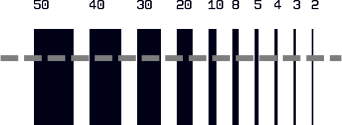
\includegraphics[width=\textwidth]{figs/fab/wiremouldprofile/lines.pdf}
    \vspace{1cm}
    \caption{}
  \end{subfigure}
  \hspace{1cm}
  \begin{subfigure}[b]{0.55\textwidth}
  \begin{tikzpicture}
    \begin{axis}[
        enlargelimits=true,
        xlabel=Scan distance (\si{\micro\meter}),
        ylabel=Height (\si{\micro\meter}),
        legend pos=outer north east,
        width=0.9\textwidth,
        height = 0.45\textwidth
    ]
    \addplot [
      color=purple,
      no marks,
      style=very thick
      ]
    table
    {figs/fab/wiremouldprofile/mould.dat};
    \addlegendentry{Mould}
    \addplot [
      color=gold,
      no marks,
      style=very thick
      ]
    table
    {figs/fab/wiremouldprofile/wire.dat};
    \addlegendentry{Wires}
    \end{axis}
  \end{tikzpicture}
    \caption{}
  \end{subfigure}
  \caption{Stylus profiling of the characterisation features. In (a) the
  characterisation lines feature of the chip is shown in detail (c.f.
  \mysubfigref{design:fig:chipexperiment}{b}) the grey dashed line denoting the
  profile. Typical profiles are shown in (b), for both the photoresist
  mould and the plated wires. Stylus size limits the size of the trenches that
  can be fully profiled, and can make both trenches and hills appear narrower
  and wider respectively.
  }
  \label{fab:fig:chipprofile}
\end{figure}

Note that when examining the trenches of the mould with the profilometer, we
must account for the finite size of the stylus.
The profilometer available at LCN is fitted with a gold stylus of radius
\SI{5}{\micro\meter}. This limits the resolution of the profile, hence why the
trenches in \myfigref{fab:fig:chipprofile} become distorted at and below
\SI{10}{\micro\meter}. This also means that the wires can appear to be 
wider, and the trenches narrower than actuality, accounting for the overlap in the
figure.

\subsection{Troubleshooting}

The electroplating procedure was initially unreliable, but we have developed
it into a robust process. It is of use to note some of the complications
that we experienced and how they were overcome. 

% See OneNote 27 Nov 2019
Our first attempt at electroplating was with the underexposed early design
photoresist mould shown in \mysubfigref{fab:fig:moulds}{a}, meaning that the
full wires could not have been formed. These were nonetheless suitable targets
for practice. We manually agitated the electroplating solution during plating
and were successful in laying down the larger features such as the wire bond
pads, but sub $\sim100\si{\micro\meter}$ features were not formed, as could be
seen after removing the photoresist mould. This is shown in 
\mysubfigref{fab:fig:aggandcorr}{a}.

We attempted to improve the adhesion with manual agitation in combination with
a bubbler, but eventually found that we achieved the best results with a
combination of gentle stirring by a magnetic stirrer in combination with
bubbling of the Goldbath. This allowed us to fabricate the smallest features
resolvable in the mould.  
%
For later attempts at electroplating we ensured the mould had been exposed and
developed correctly, such as the one shown in \mysubfigref{fab:fig:moulds}{b}.
With these moulds we were able to reliably fabricate features below the
\SI{10}{\micro\meter} scale.

Next, the photoresist must be removed. We initially attempted this by 
sonicating in acetone for twenty minutes, however this resulted in the debris
visible in \mysubfigref{fab:fig:aggandcorr}{b}. It was resolved that acetone was
unsuitable and Dow Electronic Materials Microposit Remover 1165 heated to
\SI{65}{\celsius} was used instead.
%
Examples of photoresist removal by this procedure are shown in
\mysubfigref{fab:fig:aggandcorr}{c} and (d). Here it can be seen that clear
wires have been achieved, but the small wires have been damaged by sonicating.
Sonicating can be avoided by instead soaking the dies in the Microposit Remover
1165 overnight at room temperature.

\begin{figure}
  \centering
  \begin{subfigure}[b]{0.45\textwidth}
  \begin{overpic}[width=\textwidth]{figs/fab/eplatetroubleshoot/aggandcorr/manualagg_flipped_scale.png}
    \put(70,67){\SI{50}{\micro\meter}}
    \put(10, 70){(a)}
  \end{overpic}
  \end{subfigure}
  \hspace{1cm}
  \begin{subfigure}[b]{0.45\textwidth}
    \centering
    \begin{overpic}[width=\textwidth]{figs/fab/eplatetroubleshoot/aggandcorr/corrosion_flipped_scale.png}
    \put(6,67){\SI{50}{\micro\meter}}
    \put(85, 70){(b)}
  \end{overpic}
  \end{subfigure} \\[0.5cm]
  \begin{subfigure}[b]{0.45\textwidth}
    \centering
    \begin{overpic}[width=\textwidth]{figs/fab/eplatetroubleshoot/aggandcorr/goodpads_scale2.png}
      \put(75,6){\textcolor{white}{\SI{50}{\micro\meter}}}
      \put(10, 70){\textcolor{black}{(c)}}
  \end{overpic}
  \end{subfigure}
  \hspace{1cm}
  \begin{subfigure}[b]{0.45\textwidth}
    \centering
  \begin{overpic}[width=\textwidth]{figs/fab/eplatetroubleshoot/aggandcorr/goodcentre_scale.png}
      \put(10, 70){\textcolor{black}{(d)}}
    \put(69,10){\SI{50}{\micro\meter}}
  \end{overpic}
  \end{subfigure}
  \caption{
    Electroplating problems and solutions.
    Microscope images showing the effects of insufficient agitation (a) and
    removal of the photoresist with solvents (b) can be compared to later
    results, where the solution is well agitated during electroplating (c) and
    the photoresist is removed with Microposit Remover 1165. Subfigure (d)
    shows the central features of the die same shown in (c), highlighting the
    damage caused by sonicating. All three dies here have been electroplated at
    \SI{10}{\milli\ampere} for \SI{200}{\second}, and use the early
    iteration of the design shown in \myfigref{fab:figs:earlydesign}.
  }
  \label{fab:fig:aggandcorr}
\end{figure}

After several iterations of electroplating we found that the larger wires were
not uniformly plated, with some areas near the edge seemingly shadowed by the
mould as shown in \myfigref{fab:fig:shadow}. This phenomenon was also noted in
\inlineref{Treutlein2008}, where it is suggested that the only solution is to
change to a new batch of Goldbath-SF. Indeed doing this and following the same procedure
produced results without this shadowing effect.
%
% This is likely due to aging, as we started to see the effect after coming
% back from covid.
%
We noted that the plating rate with the new batch of solution was not
consistent with what we had seen previously, suggesting some variation in
plating efficiency between batches.

\begin{figure}[h]
  \centering
  \begin{subfigure}[b]{0.4\textwidth}
  \begin{overpic}[width=\textwidth]{figs/fab/shadowing/scan.png}
    \put(78,11){\color{white} \SI{50}{\micro\meter}}
  \end{overpic}
    \vspace{0.7cm}
    \caption{}
  \end{subfigure}
  %\hspace{1cm}
  \begin{subfigure}[b]{0.55\textwidth}
  \begin{tikzpicture}
    \begin{axis}[
        enlargelimits=true,
        xlabel=Scan distance (\si{\micro\meter}),
        ylabel=Height (\si{\micro\meter}),
        width=0.9\textwidth,
        height = 0.7\textwidth
    ]
    \addplot [
      color=gold,
      no marks,
      style=very thick
      ]
    table
    {figs/fab/shadowing/shadow.dat};
    \end{axis}
  \end{tikzpicture}
    \caption{}
  \end{subfigure}
    \caption{
      The importance of a fresh bath. For large features
      ($>50\si{\micro\meter}$) we sometimes observe this `shadowing' effect,
      shown here on the \SI{200}{\micro\meter} wire of \ph{design 2}. this can
      be seen as a gradual gradient on the microscope (a), and confirmed with
      stylus profiling (b). The profile is taken in the direction and position
      of the white dotted line shown in (a). Changing to fresh golbath solution
      resolves this problem.
    }
  \label{fab:fig:shadow}
\end{figure}

\section{Etching}

The seed layer electrically connects the trapping wires, which is
essential for electroplating, but it must be removed to separate the wires
during operation. We do this by etching the chip to remove the height of the
seed layer from the entire surface. Since the seed layer is only a few tens of
nanometres and the wires are on the scale of micrometers, the effect of the
etch on the wires is negligible.

Any thin films or other debris left on the die can become stuck to the chip
during etching, so it is essential to ensure that the die is very well cleaned
having been electroplated outside the cleanroom.  We found that a solvent clean
on its own was insufficient, and would leave some debris on the die after the
etch that we could not remove, shown in \myfigref{fab:fig:etchres}. This was
resolved by also cleaning for ten minutes in an oxygen plasma, suggesting that
this debris may have been caused by residual photoresist.

% TODO Need a scale on these figures
% TODO Should I highlight and say something about the deformity due to the bead
% too?
\begin{figure}
  \centering
  \begin{subfigure}[b]{0.35\textwidth}
    \begin{tikzpicture}
    \node[anchor=south west,inner sep=0] at (0,0)
{ 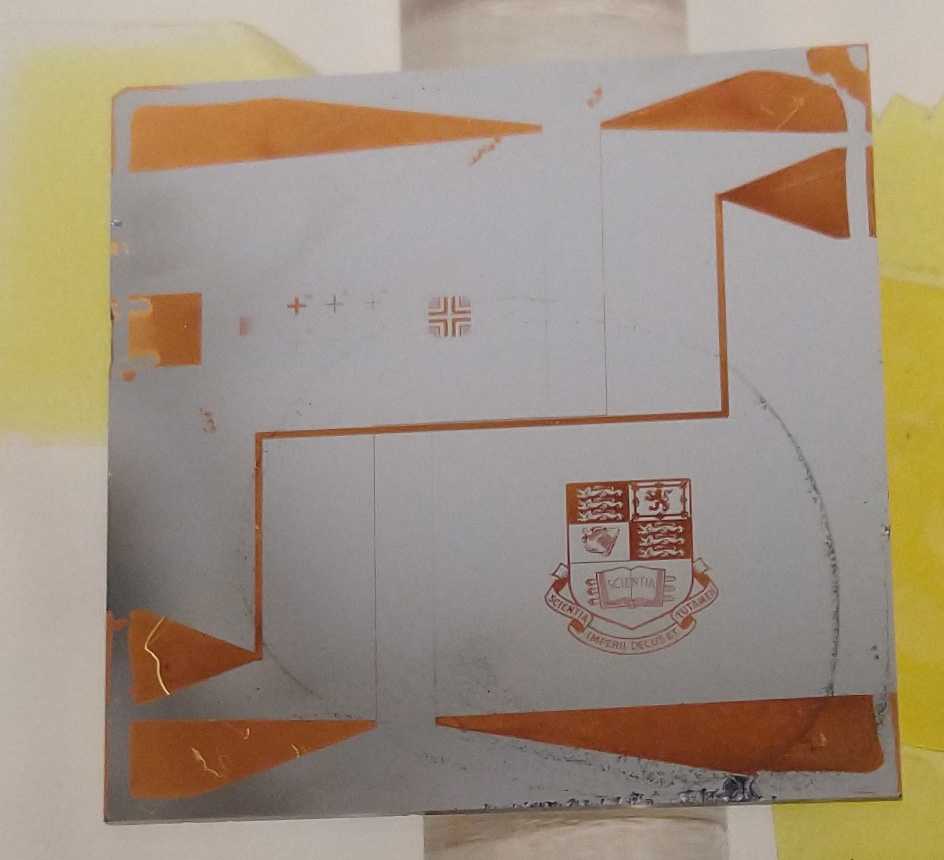
\includegraphics[width=\textwidth]{figs/fab/etch/etchdebris.jpg} };
    \draw[red,ultra thick,rounded corners] (5,3.5) rectangle (5.8,5.3);
\end{tikzpicture}
    \caption{}
  \end{subfigure}
  \hspace{2cm}
  \begin{subfigure}[b]{0.35\textwidth}
    \centering
  \begin{overpic}[width=\textwidth]{figs/fab/etch/etchdebris_scope_crop_scale.png}
    \put(67,14){\SI{100}{\micro\meter}}
  \end{overpic}
    \caption{}
  \end{subfigure}
  \caption{Debris left on the die after etching. It was found that this can be
  avoided by cleaning with an oxygen plasma for ten minutes prior to etching.
  Macroscopic view of the entire chip is shown in subfigure (a), where the red
  box also highlights malformed features due to the photoresist bead. Detail of
  debris near the wires is shown in the microscope image in subfigure (b).}
  \label{fab:fig:etchres}
\end{figure}

After cleaning, the gold is etched away by  by placing the chip into a beaker
of etchant. We used a pre-mixed etchant made up of 50\% potassium iodide and
\numrange{10}{20}\% iodine, which is pre-mixed by Sigma-Aldrich. This etches
gold at a rate of \SI{5}{\nano\meter\per\second}, so an etch of
\SIrange{5}{10}{\second} will remove the seed layer. After this the chip is
immediately transferred to a beaker of deionised water and then rinsed.  Visual
inspection of the die will clearly show if the seed layer has been removed.

To complete the separation of the wires, the chromium layer must also be etched
in the same way. For this we use another Sigma-Aldrich pre-miexed etchant of
\numrange{20}{25}\% diammonium hexanitritratocerate and \numrange{5}{10}\%
nitric acid. The process is the same as for the gold etch: the chip is
submerged in a beaker of the etchant and after \SIrange{2}{5}{\second} it is
transferred to deionised water and then rinsed. This stage of the fabrication
is represented in \mysubfigref{fab:fig:process}{10}. 

We occasionally found that etching could cause some of the smaller features to
become detached from the chip, see \myfigref{fab:fig:overetch}. This could
be due to over-etching, or poor adhesion from electroplating. To overcome this
we made changes to the chip design, making the central wire larger (the Z2 wire
was originally only \SI{4}{\micro\meter} in width) and adding the anchoring
pads shown in \mysubfigref{design:fig:chipexperiment}{b}. It is helpful when
etching to be very careful with the chip, and hold it in the etchant with
tweezers as opposed to dropping it. This ensures that the die can be removed
and placed into water without delay -- particularly important when the etching
time is only a few seconds.

% Data from Fab/characterisation/2021-03-16/G
\begin{figure}
  \centering
  \begin{subfigure}[b]{0.35\textwidth}
    \centering
    \begin{overpic}[width=\textwidth]{figs/fab/overetch/crosses_scale.jpg}
      \put(66,10){\SI{200}{\micro\meter}}
  \end{overpic}
    \caption{}
  \end{subfigure}
  \hspace{1cm}
  \begin{subfigure}[b]{0.35\textwidth}
    \centering
    \begin{overpic}[width=\textwidth]{figs/fab/overetch/centre_scale2.jpg}
      \put(66,10){\SI{200}{\micro\meter}}
  \end{overpic}
    \caption{}
  \end{subfigure}
  \caption{Microscope images showing features detached from the chip after
  etching. In subfigure (a) we can see that a \SI{5}{\micro\meter}
  characterisation cross has become detached and drifted on to the
  \SI{10}{\micro\meter} cross. Similarly, the small wire has become detached
  from the susstrate in subfigure (b). This could be due to over-etching or
  poor adhesion at an earlier stage of the process.}
  \label{fab:fig:overetch}
\end{figure}

\section{Inspecting the finished die}

To ensure that the etches have been successful, stylus profiling is once again
performed. We ensure that the wires are of a sufficient height and width to
achieve the required currents as detailed in chapter~\ref{design}. Visual
inspection under an optical microscope is also useful to ensure that the
silicon dioxide has been completely exposed. A multimeter is used to confirm
that there is continuity across the wires.

\begin{figure}
\centering
  \begin{subfigure}[c]{0.45\textwidth}
  %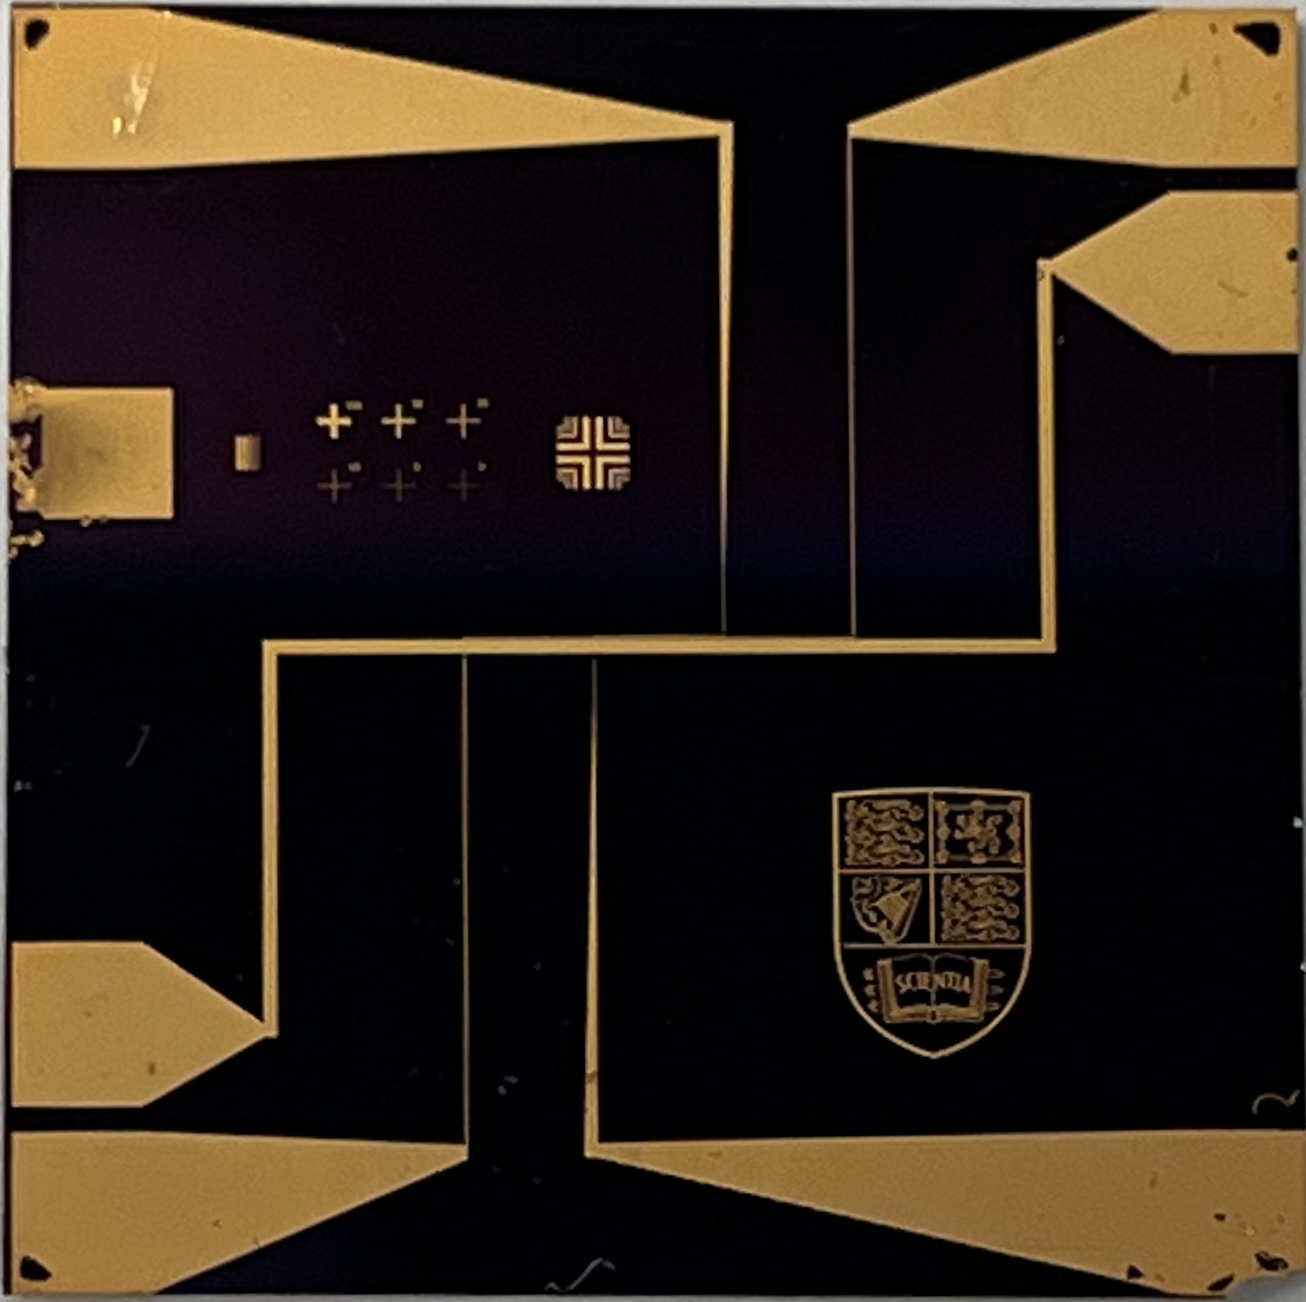
\includegraphics[width=0.8\textwidth]{figs/fab/zeta/wide_crop.jpg}
    \begin{overpic}[width=0.8\textwidth]{figs/fab/zeta/wide_crop.jpg}
      \put(3,90){\textcolor{black}{(a)}}
  \end{overpic}
  \end{subfigure}
  \begin{subfigure}[c]{0.45\textwidth}
  %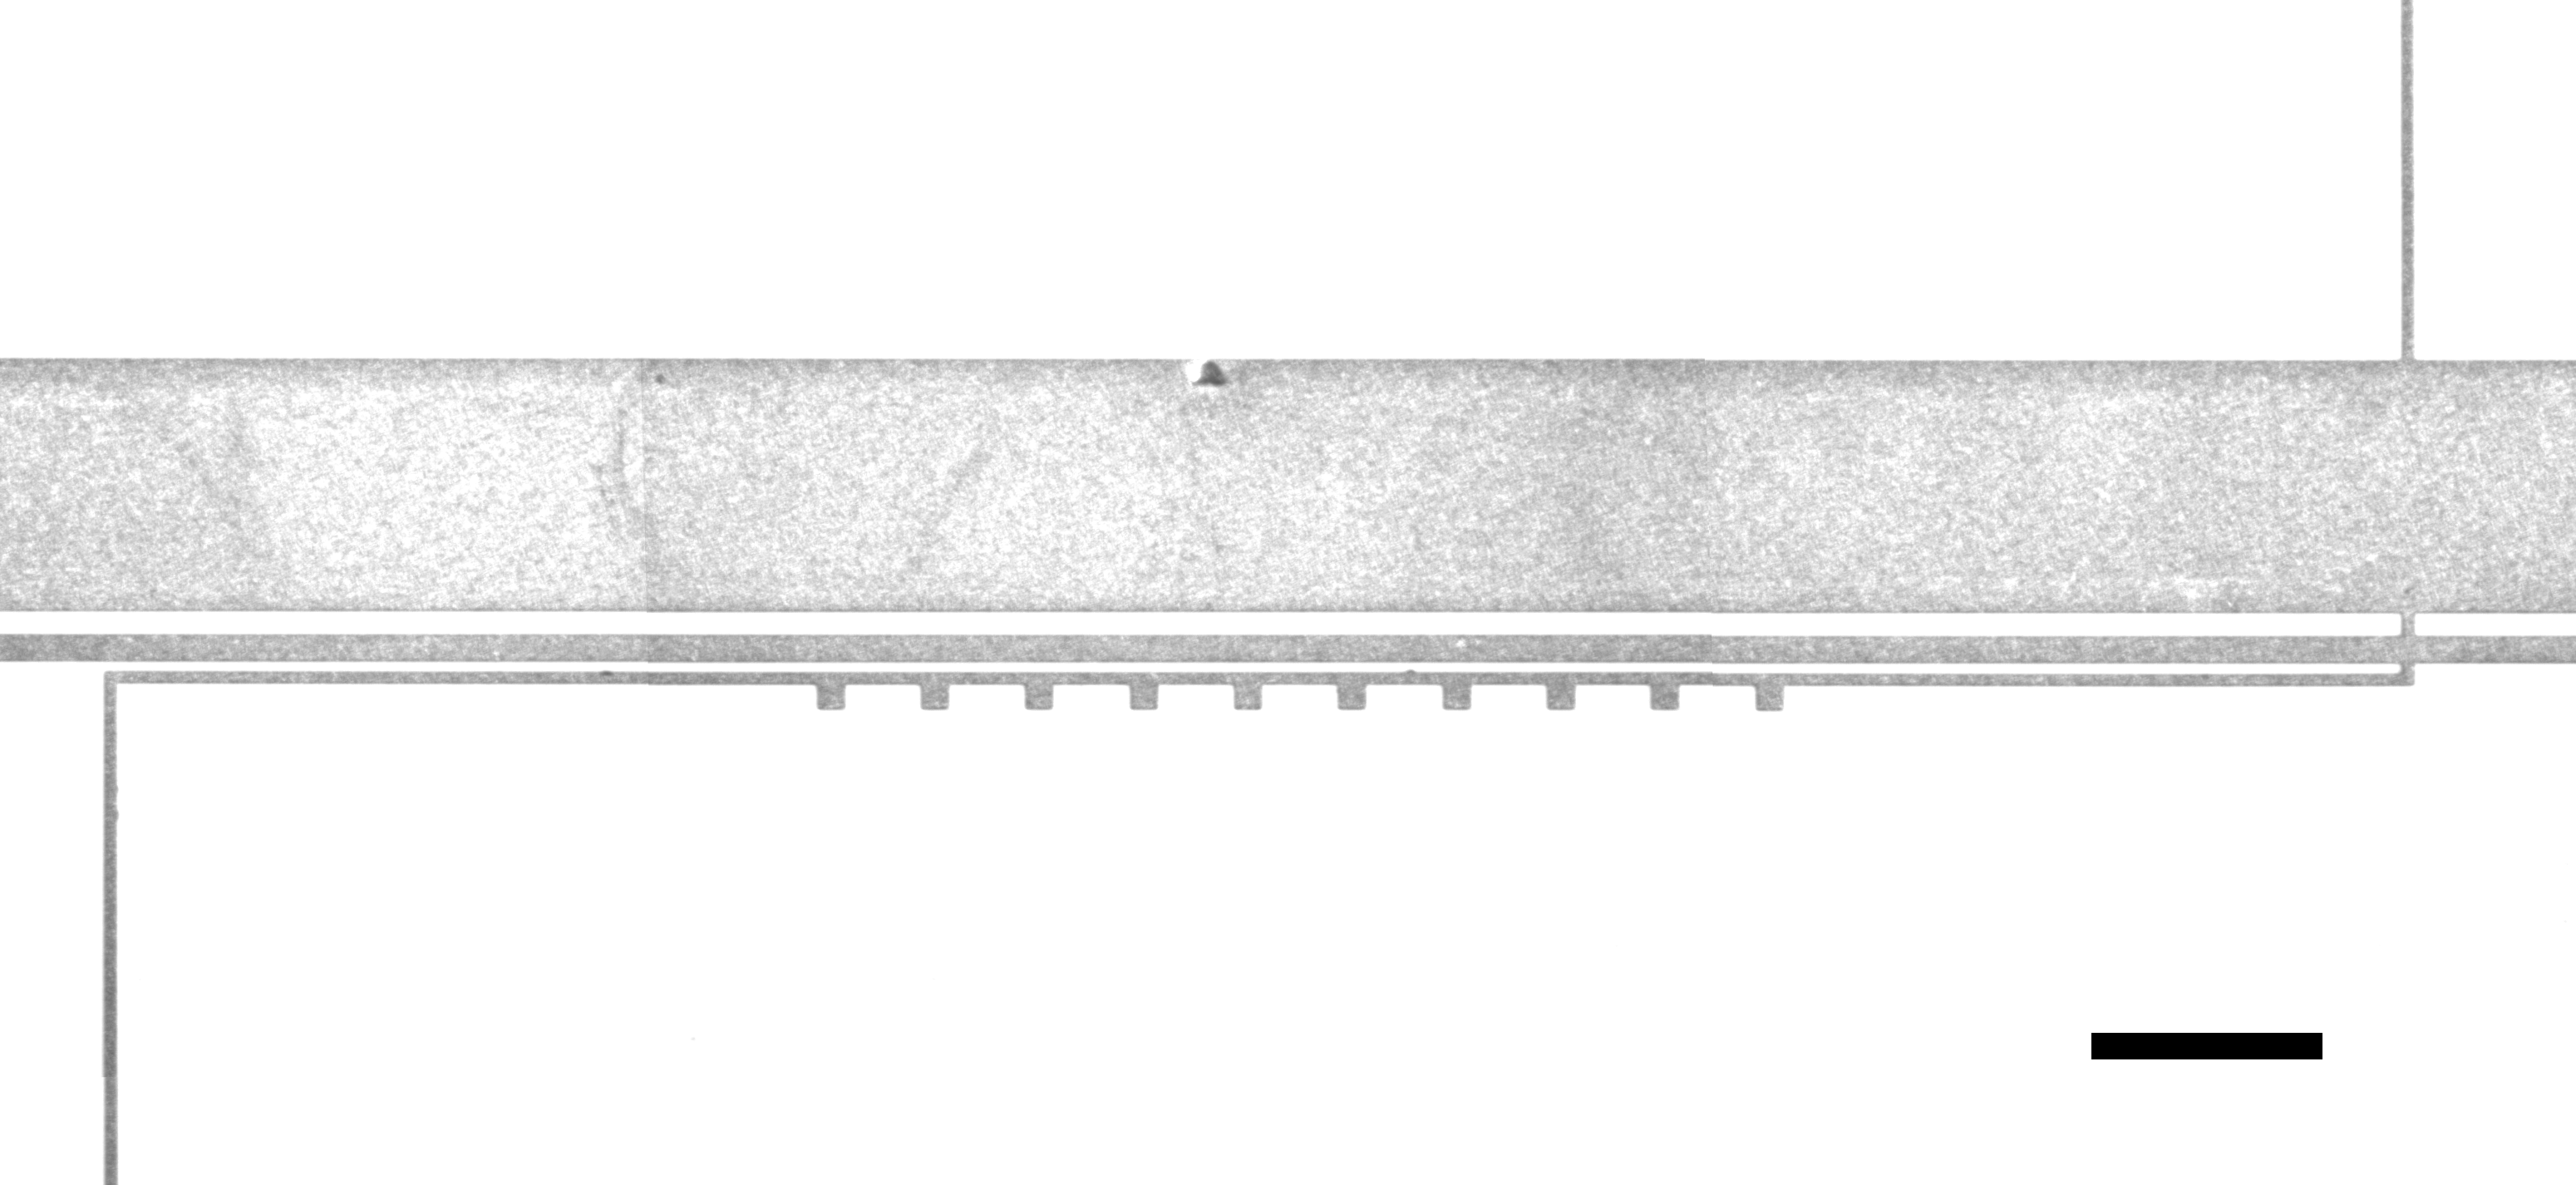
\includegraphics[width=0.8\textwidth]{figs/fab/centrestitch/centre_scale.png}
    \begin{overpic}[width=0.8\textwidth]{figs/fab/centrestitch/centre_scale.png}
      \put(3,63){(b)}
      \put(80,10){\SI{200}{\micro\meter}}
  \end{overpic}
  \end{subfigure}
  \caption{Macroscopic (a) and microscopic (b) images of a completed chip. The wires are plated to a
  height of \SI{5}{\micro\meter} and the profile of the characterisation lines
  is shown in \myfigref{fab:fig:chipprofile}}
  \label{fab:fig:zeta}
\end{figure}

\section{Connection to subchip}

% Check when I introduce initials here, could be in ch 1 or smth
To be used in the molecule experiment, the die must be mounted on the subchip
described in section~\ref{design:overview} and electrical connections made. We
attempted two methods of doing this, first we tried a combination of gluing the
die into the subchip and making connections with wirebonds. We later found that
the wirebonds failed before reaching the requried current, and therefore were
unsuitable (see \cm{section in
experiment chapter}). Alternatively it is possible to solder directly between
the die and the subchip, in this case gluing is not required to hold the chip
in place.

\subsection{Gluing and wirebonding}

For the glue, we use Epoxy Technology H77, a two-component UHV compatible epoxy
with good thermal conduction.  The two parts of the epoxy are mixed in a five
to one ratio by weight using a mass balance, and then a tiny amount is applied
to the subchip. Only enough epoxy is required that when the die is pressed onto
the surface there will be a meniscus between the surfaces of the die and the
subchip.

The epoxy is pipetted into the mounting hole, and the die placed on top. This
is followed by pressing in a vacuum bag, evenly pushing the die into the epoxy
and helping to remove air pockets in the epoxy, which could result in
virtual leaks under vacuum conditions.
%
Finally the chip and subchip are removed from the bag for baking at
\SI{115}{\celsius} for an hour and left to cool. Vacuum testing of the glue is
described in \cm{a later section}.

After gluing the chip into place, an electrical connection can be formed by
wirebonding. In this process a thin wire is attached between the subchip and
the chip by ultrasonic bonding. An overview of the process is available in
\inlineref{Harman2010}. In our case we used gold wires with
\SI{25}{\micro\meter} diameter wires and the Kulicke and Soffa 4523 wedge
bonder at LCN. It was possible to reliably produce eight bonds on each pad,
which was limited by the width of the pad and the size of the bonding head.

\subsection{Soldering connections}

The second method of connection was to place the die into the subchip and then
solder the connection between the traces on the subchip and the wirebond pads
on the chip. This was initially attempted with a UHV compatible soldering
method. We used isopropyl alcohol soluble solder flux made by Accu-Glass
Products, and gold-tin wire from Goodfellow Cambridge Ltd.\ (80\% gold, 20\%
tin) as solder. The idea is that the UHV compatible flux can be removed by
sonicating in isopropyl alcohol, removing any components that may outgas under
vacuum.

We found that using this method it was possible to create good bonds between
the chip and the subchip, however doing so was highly unreliable. The solder
does not easily flow onto the subchip traces, seemingly because a soldering
iron will not heat it sufficiently. We attributed this to the aluminium-core
PCB acting as a heat sink, and overcame the issue by using a hotplate to heat
the PCB in addition to using a soldering iron. This allowed us to reach
sufficiently high  local temperatures at the solder joint.
%
However, this had the detrimental effect of causing the wirebond pads on the
chip to come loose upon soldering. This only occurred when soldering with the
hotplate, so we assume that it was the high temperatures that led to the
features detaching from the chip.

Since this was unsuccessful, it was decided to attempt soldering with standard
solder from RS Components.. This was successful, and useful for our initial current
testing (discussed in \cm{ref section}). We found that we were able to
achieve sufficiently low vacuum without using the special UHV compatible
method. Simply soldering with the RS Components solder and cleaning the subchip
assembly with IPA was sufficient to reach pressures on the order of
\SI{1E-10}{\milli\bar}, as discussed \cm{in a later chapter}. The coplted chip
mounted to the subchip is shown in \myfigref{fab:fig:mountedsubchip}.

\begin{figure}
  \centering
  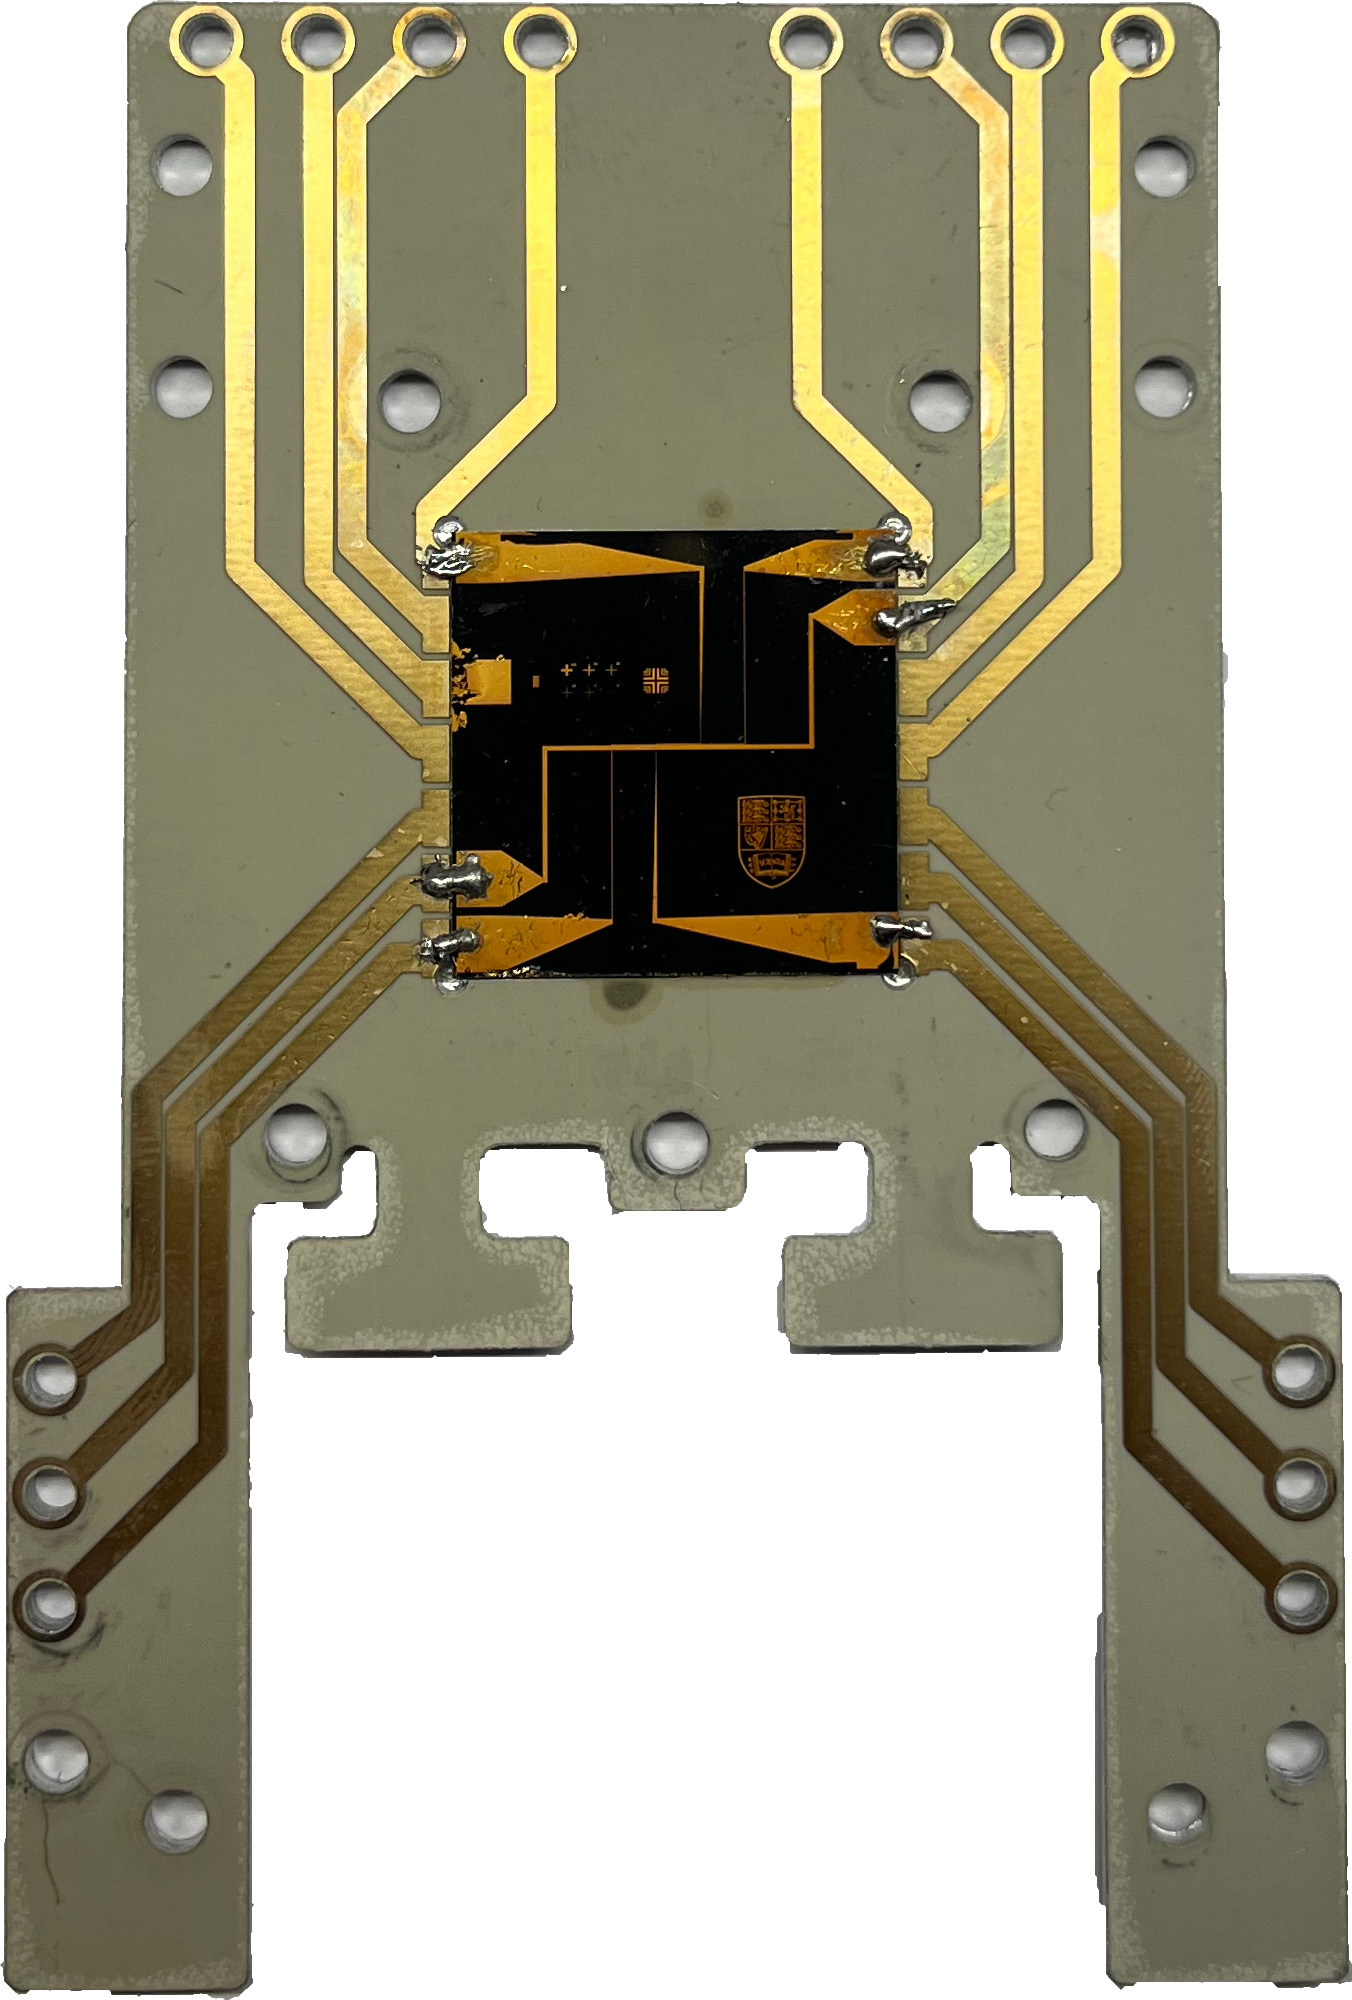
\includegraphics[width=0.4\textwidth]{figs/fab/mountedchip/mount.png}
  \caption{The chip mounted and soldered into the subchip.}
  \label{fab:fig:mountedchip}
\end{figure}

\section{Scaling fabrication}

In future design iterations it may be useful to scale the fabrication process
up by fabricating on the wafer scale rather than the scale of an individual
die. An entire wafer can be metallised, spin coated and exposed to
produce the photoresist mask. Electroplating on the wafer scale will take
longer, scaling linearly with the number of chips on the wafer. It may therefore
be beneficial to use a smaller wafer, and fabricate a few chips at a time.
Alternatively, the design could be changed so that the traps and chips are
smaller. Etching would be performed on the entire wafer before dicing into the
individual dies.

\section{Planned fabrication of microwave layer}
\label{fab:planned}

In \cm{an earlier chapter}
we described how a molecule chip could allow strong coupling between \CaF{}
molecules and a microwave field, however for this to be possible there must be
good overlap between the microwave field and the trapped
molecules~\cite{Andre2006}.

This overlap has previously been achieved for atoms in a magnetic
trap~\cite{Treutlein2008}. An insulating layer is spin coated on to the
trapping wires, upon which a CPW can be fabricated by photolithography. The
trap centre can be positioned at a resonator antinode, where the microwave
field is strongest.

Our fabrication scheme can be extended in a similar fashion. The first stage will be to spin coat the insulating layer on top of an
etched chip, as shown in \mysubfigref{fab:fig:process}{11}. Again taking our
lead from \inlineref{Treutlein2008}, we will use polyimide. Polyimide is chosen
due to its low dielectric loss tangent ($\tan\delta_e = 0.016$) which will
be discussed further in \cm{microwave chapter}.

When spin coating the polyimide it is essential that we are able to produce a
flat surface onto which we can fabricate the microwave layer. We can do this by
applying multiple layers of polyimide on the spin coater, so that any bumps are
smoothed out. This is known as planarization and is discussed further in
\inlineref{Madou2002}.

After the application of a planarized polyimide layer it will be possible to
fabricate microwave guides on the surface by lithography. The end result is
shown in \mysubfigref{fab:fig:process}{12}. We will undertake further work to
determine the required height of the CPW features and where they must be
positioned relative to the wires to achieve the strongest coupling. We will
discuss in \cm{microwaves chapter} that for a microwave resonator we must use
a superconducting CPW, or else the quality factor will be too low due to
resistive losses. The fabrication of superconducting CPWs is a well developed
field, and is discussed in for example \inlineref{doi:10.1063/1.3010859}.

